\clearpage
\section{Clock Alignment and End-to-End Message Timing}
\label{sec:gpio-clock}
Message latency requires timestamps at clearly defined boundaries and a mapping between the clocks that produced them. Offset is a difference between numerical clock readings, not a communication delay. \texttt{runOperator} does not collect these delays. The measurement command is \texttt{onDesktop/runClocksCalib}. It requires path~B: Pi Ethernet \texttt{10.0.0.120}, Pi Wi-Fi \texttt{10.0.0.20}, and Desktop Ethernet \texttt{10.0.0.2}. A shared GPIO edge aligns Pi with Teensy, and four-timestamp UDP probes align Desktop with Pi.

\subsection{Current measurement}
\label{sec:clock-method}
\texttt{runClocksCalib} leaves the wheels stopped and does not change Teensy firmware. The controller must not be running, because this command owns \texttt{/dev/serial0}. The optional \texttt{--pairs} count defaults to 100, and probes on the two paths are 25\,ms apart. The command refreshes \path{config/boot.json}, measures both network paths, then measures the timing wire. The Mac builds one summary and copies only that file to \path{/home/pi/plant_lineFollower/config/clock_calib.json}.

The Mac--Pi half starts a \texttt{clock\_probe} server on each Pi address: Ethernet \texttt{10.0.0.120} on \texttt{eth0}, port 53120, and Wi-Fi \texttt{10.0.0.20} on \texttt{wlan0}, port 53121. Desktop binds \texttt{10.0.0.2} and alternates probes between those servers. Each probe records Desktop send $D_1$, Pi receive $P_2$, Pi reply $P_3$ and Desktop receive $D_4$. Pi turnaround is removed from the corrected round trip,
\begin{equation}
R_{DP}=(D_4-D_1)-(P_3-P_2).
\label{eq:clock-corrected-rtt}
\end{equation}
The saved half-width of a probe is half of that corrected round trip. It is a single-probe bound, not an intersection of many probes. The saved midpoint is the Desktop$-$Pi clock origin, not a network delay. One-way delay is not obtained by splitting the round trip in half. For each path the summary keeps the valid and failed counts, the minimum and median corrected round trip, and the median half-width and midpoint.

The Pi--Teensy half then runs \texttt{gpio\_clock} for 200 rising edges at up to 20\,Hz. Teensy pin 20 drives Pi GPIO23 through 5\,k$\Omega$. Three 0.5\,s flashes on both LEDs check the wire and are excluded from the fit. The offset convention is Pi time minus Teensy time. The summary keeps whether the run completed, the valid and requested edge counts, standby confirmation, the first-pulse offset, the nominal offset at the Pi reference time, the quartiles of the change from the first pulse, the fitted drift in ppm, the detrended residual range, the maximum Teensy write bracket, and the median delay from the kernel edge into the Pi process. That userspace delivery delay is not part of the offset.

Individual probes and individual edges are discarded after the summary is written. The file copies \texttt{hash8} from \path{config/boot.json} and adds the Pi local time and \texttt{uptime\_s}. A later reboot writes a new \path{boot.json}. Section~\ref{sec:init-datagram} sends this file to the operator in the initialization datagram. The operator uses it only when the two \texttt{hash8} values match; a robot run then takes the Wi-Fi half-width, not the Ethernet one. Equation~\eqref{eq:transmit-uncertainty} is the uncertainty reported from that summary.

\subsection{Path-B summary on October 11, 2026}
\label{sec:clock-delay-current}
One default \texttt{runClocksCalib} run, 100 pairs, was taken with the robot idle and the motors stopped. The Pi boot \texttt{hash8} was \texttt{f03276bd}. The summary was written at Pi local time 2026-10-11T11:07:22$-$07:00, with \texttt{uptime\_s} $=2201.95$. All 200 Mac--Pi probes were valid, 100 on each path, and all 200 Pi--Teensy edges were valid. The summary does not store a round-trip maximum. The Desktop$-$Pi midpoint was $5.13328376\times 10^{8}$\,ms on Ethernet and $5.13328377\times 10^{8}$\,ms on Wi-Fi; both are clock origins, not delays.

\begin{table}[H]
\centering
\caption{Mac--Pi corrected round trip and offset half-width, in milliseconds, from \protect\path{config/clock_calib.json} on October 11, 2026. Each half-width is half of that probe's corrected round trip. These are single-probe bounds. A robot run uses only the Wi-Fi half-width.}
\label{tab:clock-delay-current}
\begin{tabular}{lrrrr}
\toprule
Path & Valid & RTT min & RTT median & Half-width median \\
\midrule
Ethernet & 100 & 0.740 & 0.999 & 0.500 \\
Wi-Fi & 100 & 1.644 & 2.072 & 1.036 \\
\bottomrule
\end{tabular}
\end{table}

The Pi--Teensy half completed 200 of 200 edges and confirmed standby. The first-pulse Pi$-$Teensy offset was $-5.530234$\,s, and the nominal offset at Pi reference time 2193.042\,s was $-5.530222$\,s. Change from the first pulse had quartiles $+5$, $+12$ and $+19$\,$\mu$s. The fitted drift was 2.739\,ppm and the detrended residual range was 37.7\,$\mu$s. The Teensy write bracket never exceeded 1\,$\mu$s. Median delivery of the kernel edge into the Pi process was 138\,$\mu$s; that delivery delay is not part of the offset. The same file was sent to the operator for the run in Section~\ref{sec:init-datagram}.

The numerical results after this subsection are stale. They come from earlier captures, including full probe and edge archives that the current command does not keep.

\subsection{Stale path-B result from October 11, 2026}
\label{sec:clock-delay-20261011}
\textbf{Stale.} This shorter run used \texttt{runClocksCalib --pairs 40} and kept the full Mac and Pi archives named below. It is not the summary now written to \path{config/clock_calib.json}.

\begin{table}[H]
\centering
\caption{Stale. Mac--Pi corrected round trip and raw offset half-width, in milliseconds, October 11, 2026. Each half-width is half of that probe's corrected round trip. These are single-probe bounds, not the expanded intersection used for the September 28 session later in this appendix. The Desktop$-$Pi midpoint was about $4.968\times 10^{8}$\,ms on both paths; that value is the difference of clock origins, not a network delay.}
\label{tab:clock-delay-20261011}
\begin{tabular}{lrrrrr}
\toprule
Path & Probes & RTT min & RTT median & RTT max & Half-width median \\
\midrule
Ethernet & 40 & 0.706 & 0.970 & 2.799 & 0.485 \\
Wi-Fi & 40 & 1.621 & 2.110 & 9.398 & 1.055 \\
\bottomrule
\end{tabular}
\end{table}

The Pi--Teensy half of this stale run used 200 rising edges at up to 20\,Hz after three 0.5\,s LED flashes. The first-pulse Pi$-$Teensy offset was $-5.483318$\,s, again a clock-origin difference. Change from that first pulse had quartiles $+10$, $+19$ and $+27$\,$\mu$s. The fitted drift was 3.008\,ppm and the detrended residual range was 71.5\,$\mu$s. The Teensy write bracket never exceeded 1\,$\mu$s. Median delivery of the kernel edge into the Pi process was 152\,$\mu$s; that delivery delay is not part of the offset. The Mac records are \path{lineFollowerDistributedBin/out/clocks/20261011_063747/}. The Pi record is \path{lineFollowerDistributedBin/out/pi_teensy_clock.latest.json}, archived as \path{out/raspberry_pi/pi_teensy_clock_20261011_061014_1144.json}.

The subsections below keep the September 27--28 recordings and the earlier per-job procedure. Their numbers are stale as well. The shared-edge and four-timestamp definitions are the ones \texttt{runClocksCalib} still uses; the launch, the saved file and the lack of a per-job repeat are the current method in Section~\ref{sec:clock-method}.

\subsection{Pi--Teensy Alignment Using a Shared GPIO Edge}
\subsubsection{Purpose and Wiring}
Before subtracting a UART send timestamp on one processor from a receive timestamp on the other, their clocks must be aligned. The measurement uses a shared GPIO edge for the \emph{Pi--Teensy clock offset}. It measures clock offset, not UART transit time. The September 27 controller runs below used this map; a robot run started by \texttt{runOperator} no longer collects it. Unlike a ping-based estimate, it does not require equal communication delays in the two directions: both processors observe the same electrical event, and UART subsequently transports the timestamp record.

Figure~\ref{fig:pi-teensy-tb6612-wiring} shows the installed timing connection: \textbf{Teensy pin 20 output $\rightarrow$ 5\,k$\Omega$ $\rightarrow$ Pi GPIO23 input (physical header pin 16)}, with common ground and 3.3\,V signaling. The green indicator uses Pi GPIO24 (header pin 18); the white indicator uses Teensy pin 21, each through a separate 5\,k$\Omega$ resistor to its grounded LED. UART remains Pi GPIO14/TX (header 8) to Teensy RX1/pin 0, and Teensy TX1/pin 1 to Pi GPIO15/RX (header 10), at 115200 baud, 8N1.

\subsubsection{Measurement Procedure and Timestamp Meaning}
The test stops ADC streaming and keeps both motors disabled. At startup Teensy raises its LED and the timing wire together; Pi mirrors the detected edges to its LED. Both LEDs flash twice, each time 0.5\,s on and 0.5\,s off. This provides a visible wiring check; the four startup edges are excluded from timing statistics. The recorded intervals were within 0.014\,ms of 500\,ms in the two long runs. Pi's LED write followed the kernel edge timestamp by approximately 0.18--0.23\,ms, so the flashes are visually synchronized, not simultaneous electrical outputs.

Pi then requests one numbered pulse at a time, at up to 20\,Hz. A random session identifier and strictly increasing sequence number associate each GPIO event with exactly one UART record. On Teensy, interrupts are briefly masked while the firmware reads its extended 64-bit microsecond clock immediately before raising pin 20 and again after a register barrier and GPIO readback. These readings, $T_i^-$ and $T_i^+$, bracket the software output operation. The pin stays high for 2\,ms with interrupts enabled, returns low, and Teensy sends the session, sequence and timestamps over UART. Its microsecond counter is extended across 32-bit wrap; neither processor's clock is reset.

Pi uses the Linux GPIO v2 character-device interface on \texttt{/dev/gpiochip0}. It reads the kernel-provided edge timestamp $P_i$, in \texttt{CLOCK\_MONOTONIC} nanoseconds, rather than timestamping when its process wakes up. The default event clock and buffered event semantics are documented in the \href{https://www.kernel.org/doc/html/latest/userspace-api/gpio/gpio-v2-get-line-ioctl.html}{Linux GPIO line-request API} and \href{https://www.kernel.org/doc/html/latest/userspace-api/gpio/gpio-v2-line-event-read.html}{edge-event API}. No debounce or hardware timestamp engine is requested. Missing or extra edges, session/sequence mismatches, duplicate replies and timeouts invalidate the attempt and stop the run instead of shifting subsequent pairings.

All reported offsets here use the current convention
\begin{equation}
 \theta_i = \frac{P_i}{1000}-\frac{T_i^-+T_i^+}{2}
 \qquad [\mu\mathrm{s}], \qquad \theta=\text{Pi time}-\text{Teensy time}.
\end{equation}
A positive value means Pi's numerical clock reading is ahead. The approximately 2188\,s offset reflects different clock origins; it is not a transmission delay. Console progress reports the smaller change $\theta_i-\theta_1$, which can have either sign. Archived JSON schema 1 used the opposite sign; the analysis below converts it to this convention. Schema 2 and the current CSV name the convention explicitly. Raw timestamps are unchanged.

\subsubsection{Software and Reproduction}
The current Pi timing program is \path{lineFollowerDistributed/gpio_clock.cpp}, started by \texttt{runClocksCalib} for 200 edges. That command keeps only the summary fields in Section~\ref{sec:clock-method}. The archived captures below were taken with the earlier standalone program \path{measure_pi_teensy_clock} and are stale. Teensy runs Arduino C++ in \path{lineFollowerDistributed/firmware/halo_teensy_firmware/halo_teensy_firmware.ino}, firmware revision 16, with the \texttt{GPIO\_EDGE\_CLOCK} diagnostic commands. C++ gives direct access to Linux GPIO/UART calls and Teensy GPIO registers, avoids an interpreter in the acquisition path, and matches the existing controller implementation. It does not make Linux scheduling deterministic: precision here primarily comes from the kernel event timestamp and the Teensy write bracket.

The stale September captures were run on Pi, with other UART clients stopped:
\begin{verbatim}
cd ~/robot0
./measure_pi_teensy_clock
./measure_pi_teensy_clock --samples 1000 --label idle
./measure_pi_teensy_clock --samples 1000 --cpu-load --label cpu-load
\end{verbatim}
That older default was 200 pulses, taking about 12\,s including the flashes. It printed progress and summary statistics, saved \path{out/pi_teensy_clock.latest.json} and \path{out/pi_teensy_clock.latest.csv}, and retained timestamped captures under \path{out/raspberry_pi/}. Those JSON files include raw edges, UART records, timestamps, errors, LED transitions, fit statistics and final motor-standby confirmation. The optional load was one busy C++ worker on Pi, not a full reproduction of moving-robot or network activity. The offline report script \path{docs/tools/plot_gpio_clock.py} uses Python's standard library to read these saved records and bin the data; PGFPlots renders the histogram. Python is not involved in acquiring the measurements.

\subsubsection{Measured Results and Distribution}
Table~\ref{tab:gpio-clock-results} compares two completed runs collected on September 27, 2026. Both matched all 1,000 requested pulses and confirmed motor standby afterward. Each fit uses
\begin{equation}
 \theta_i=\theta_{\rm ref}+b(t_i-t_{\rm ref})+r_i,
 \qquad t_i=P_i/10^9 \quad [\mathrm{s}].
\end{equation}
Here $b$ is in $\mu$s/s, numerically ppm, and $r_i$ is the residual after removing a least-squares line. Figure~\ref{fig:gpio-clock-histogram} plots all residuals from these runs; it does not omit outliers. The raw offsets change during acquisition, so a histogram without removing drift would mix timestamp variation with relative clock-rate mismatch.

\begin{table}[H]
\centering\small
\caption{Stale. Shared-edge clock measurement, September 27, 2026, normalized to Pi minus Teensy. Each reference time is Pi \texttt{CLOCK\_MONOTONIC}, not wall time.}
\label{tab:gpio-clock-results}
\begin{tabular}{@{}L{8.3cm}rr@{}}
\toprule
Quantity & Idle & CPU load \\
\midrule
Matched / requested edges & 1000 / 1000 & 1000 / 1000 \\
Elapsed time, including startup (s) & 52.98 & 53.47 \\
Pi reference time (s) & 2282.586009 & 2491.321708 \\
Nominal Pi--Teensy offset at reference (s) & 2188.464122723 & 2188.464834611 \\
Fitted drift ($\mu$s/s = ppm) & +3.339 & +3.186 \\
Residual Q1 / median / Q3 ($\mu$s) & -1.9 / -1.1 / +0.1 & -1.6 / -0.6 / +0.4 \\
Residual minimum / maximum ($\mu$s) & -5.5 / +67.9 & -7.4 / +34.2 \\
Residual full range ($\mu$s) & 73.4 & 41.6 \\
Maximum Teensy bracket ($\mu$s) & 1.0 & 1.0 \\
Median kernel-event-to-userspace delay ($\mu$s) & 147.0 & 156.0 \\
\bottomrule
\end{tabular}

\end{table}

\begin{figure}[H]
\centering
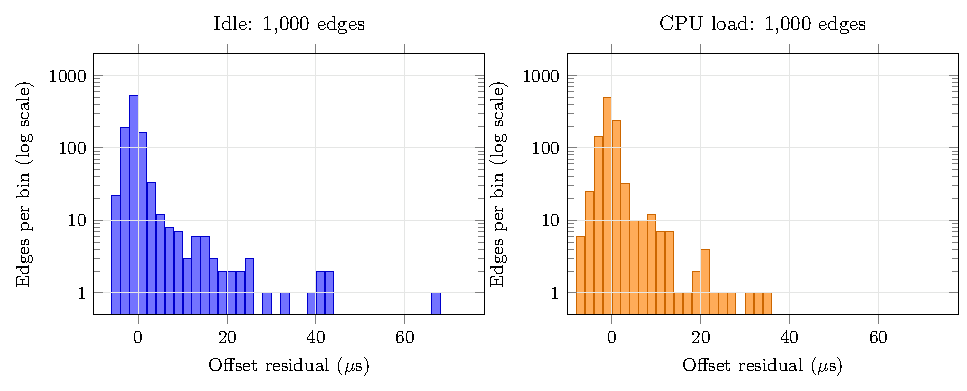
\includegraphics[width=.94\linewidth]{figures/gpio_clock/histogram.pdf}
\caption{Stale. Pi-minus-Teensy offset residuals after removing each run's fitted offset and drift, September 27, 2026. Common 2\,$\mu$s bins and logarithmic counts expose the small positive tails. Each panel contains all 1,000 valid pulses; empty bins are omitted. These are clock-measurement residuals, not UART-delay distributions.}
\label{fig:gpio-clock-histogram}
\end{figure}

The full residual ranges were 73.4\,$\mu$s at idle and 41.6\,$\mu$s under CPU load; the Teensy bracket never exceeded 1\,$\mu$s. The smaller range in the loaded run does not establish that load improves accuracy. Event delivery to Pi userspace had medians of 147 and 156\,$\mu$s, and maxima of 14.659 and 5.236\,ms, respectively. These delivery delays do not enter the offset calculation. The fitted relative drift, about 3.2--3.3\,ppm, corresponds to roughly 0.2\,ms per minute if that rate persists, so a fixed offset alone should not be extrapolated over long jobs.

The plotted captures, under \path{robot0/out/raspberry_pi/}, are:
\begin{itemize}
\item \path{pi_teensy_clock_20260927_164431_1292.json} (idle);
\item \path{pi_teensy_clock_20260927_164800_1323.json} (CPU load).
\end{itemize}
 The analysis stores their SHA-256 hashes, derived samples and bin counts in \path{docs/figures/gpio_clock/}. Short smoke/display checks are separate; one interrupted capture with 68 valid pulses is also excluded from this comparison. It recorded a 181.8\,$\mu$s residual range and confirmed standby, illustrating why the completed-run ranges are not universal bounds.

\subsubsection{Accuracy and UART Timestamp Boundaries}
No correction is applied for unmeasured latency. A 100\,$\mu$s allowance is retained as an engineering assumption, not a validated absolute error bound. Delay between the physical edge and Pi's kernel timestamp biases Pi-minus-Teensy upward; averaging cannot remove that bias. The bracket does not independently bound GPIO pad, input or interrupt latency. These histograms demonstrate repeatability, not proof of $\pm0.1$\,ms absolute accuracy.

With the fitted conversion $M(T)$ into Pi time, UART-path timing can be computed as $P_{\rm receive}-M(T_{\rm send})$ or $M(T_{\rm receive})-P_{\rm send}$, using consistent units. A software dispatch-to-complete-message interval includes serialization, buffering and receiver processing. The standalone GPIO reply is deliberately sent after a 2\,ms pulse, so its arrival minus the edge timestamp is not a pure UART delay. The running controller instead records actual sensor and motor-message boundaries, as defined below.

\subsection{Desktop--Teensy Alignment through Pi}
\label{sec:desktop-clock}
\subsubsection{Four Timestamps and the Combined Clock Map}
Desktop reaches Teensy through Ethernet to ASUS, Wi-Fi to Pi, and UART to Teensy. The primary alignment therefore combines two measurements: the shared-edge Pi--Teensy map above and a Desktop--Pi UDP exchange. It does not estimate the entire clock offset by dividing a Desktop--Teensy round trip in half.

Each UDP calibration probe records Desktop send time $D_1$, Pi receive time $P_2$, Pi reply time $P_3$, and Desktop receive time $D_4$, all converted to nanoseconds. Desktop and Pi use their own \texttt{CLOCK\_MONOTONIC} clocks. For an approximately constant offset $\phi=\text{Pi}-\text{Desktop}$, nonnegative delivery times imply
\begin{equation}
 P_3-D_4\ \leq\ \phi\ \leq\ P_2-D_1,
 \qquad R_{DP}=(D_4-D_1)-(P_3-P_2).
 \label{eq:desktop-pi-bounds}
\end{equation}
The interval width is the corrected network round trip $R_{DP}$. Pi's measured turnaround is removed; asymmetric network delay remains unknown. The implementation expands the bounds for the permitted clock-rate difference and intersects the intervals from 100 exchanges. Their midpoint is an estimate, not an assertion of symmetric paths. Repeated probes can remove variable queueing from the bounds, but cannot identify a fixed path asymmetry.

Let $M(T)$ be the GPIO-derived conversion of Teensy time into Pi time, including fitted relative drift. The combined conversion to Desktop time is
\begin{equation}
 \widehat D(T)=M(T)-\widehat\phi.
 \label{eq:desktop-teensy-map}
\end{equation}
For a constant-offset approximation this becomes $D-T=\theta-\phi$, with $\theta=\text{Pi}-\text{Teensy}$ as defined above. The software retains uncertainty intervals for both terms. Neither processor's clock is set or restarted, and wall-clock date/time is used only for run labels. A reboot writes a new \texttt{hash8} and requires a new \texttt{runClocksCalib}. A Teensy-only reset does not change that hash.

A second set of 100 probes traverses Desktop--Pi--Teensy and back. Teensy timestamps complete request receipt and reply construction; Desktop timestamps send and receipt. Request and response on UART are each 51 bytes including LF. These exchanges supply an independent causal consistency check and a round-trip distribution. Equal byte counts balance serial wire time, but do not prove equal buffering or network delay. This end-to-end estimate is not substituted for the tighter GPIO-plus-UDP map.

\subsubsection{Calibration Sequence, Drift and Saved Records}

\textbf{Stale procedure.} The integrated controller used to give each job a new session identifier and measure the clocks again before any motor arming. That repeat is no longer part of \texttt{runOperator}. The controller receives a job, sends the existing summary files, and arms; Section~\ref{sec:clock-method} is the measurement that produces \path{clock_calib.json}. In the old sequence, Pi ran its package-local \texttt{gpio\_clock} helper with exclusive UART ownership and released that ownership before reopening UART for the controller. One controller launch handled one job. Calibration failure, inconsistent clock mappings or a detected reset prevented normal continuation. The September numbers below belong to that procedure.

\begin{table}[H]
\centering\small
\caption{Stale. Previous calibration and LED sequence for an integrated remote job. Each flash is 0.5\,s on and 0.5\,s off. \texttt{runOperator} does not run this sequence.}
\begin{tabular}{@{}L{4.1cm}L{7.8cm}L{4.0cm}@{}}
\toprule
Phase & Measurement or action & LED indication \\
\midrule
Pi--Teensy startup & 200 shared GPIO edges at up to 20\,Hz; motors stopped & Both LEDs flash 3 times \\
Desktop calibration & 100 Desktop--Pi UDP exchanges, then 100 Desktop--Teensy end-to-end exchanges & Teensy LED flashes 2 times; Pi LED off \\
Robot job & Combine GPIO and network clock maps, check end-to-end consistency, then arm & Teensy LED continuously on \\
Stop and drift check & Stop motors; repeat 200 GPIO edges and save the pre/post pair & Run LED goes off, then both flash 3 times for calibration; both off afterward \\
\bottomrule
\end{tabular}
\end{table}

The run LED remains on for zero wheel targets and motor-disabled jobs too: it indicates an active control job. STOP or the configured duration turns it off. Teensy firmware also turns it off and stops motors after 750\,ms without a valid motor-target heartbeat; unrelated clock queries cannot keep that indication alive. The Pi controller's existing command-freshness safeguard remains independent. Ctrl-C stops the job and skips the post-run calibration, recording an incomplete pair. The GPIO stages each add approximately 13\,s; they do not consume the requested drive duration.

In that stale integrated job, the primary mapping combined Pi-minus-Teensy from GPIO with Pi-minus-Desktop from network probes. End-to-end pings provided a consistency check and round-trip measurement, without requiring UART path symmetry for the primary estimate. Its reported uncertainty included the assumed 100\,$\mu$s GPIO latency allowance, an assumed 50\,ppm error allowance for extrapolating the GPIO rate fit, and the network clock bounds. These remain conditional estimates, not a validated absolute accuracy guarantee. During the robot job, periodic Desktop--Pi probes and UART clock-anchor checks continued, and the post-run GPIO measurement supplied an additional drift estimate. \texttt{runOperator} does not repeat those probes. Section~\ref{sec:remote-control} gives the uncertainty it reports from the saved summary.

Both calibrations are written atomically to \texttt{.latest.json} files, with timestamped job archives retained:
\begingroup\sloppy
\begin{itemize}
\item Pi: \path{pi_teensy_clock.latest.json} in the configured output directory (for these recordings, \path{out/raspberry_pi/integrated_clock_jobs/} relative to \path{/home/pi/robot0/}), also copied to \path{/home/pi/robot0/out/pi_teensy_clock.latest.json}. The job wrapper contains full \texttt{pre} and \texttt{post} GPIO captures, completion/error status, Pi boot identifier and drift between their reference points.
\item Desktop directory: \path{2026_lineFollowerOperator/out/}. Its file \path{desktop_teensy_clock.latest.json} contains the GPIO summary, raw network and end-to-end probes, combined mapping and conditional uncertainty. A separate \texttt{desktop\_pi\_clock.latest.json} preserves the network calibration alone.
\end{itemize}
\endgroup
Match the \texttt{job\_session} strings before joining Pi and Desktop records from those stale jobs. The complete post-run GPIO capture remained on Pi and was joined to Desktop data during later analysis. A failed attempt was recorded explicitly and was not silently reused. The current command is different: \texttt{runClocksCalib} writes one summary, and a later robot run reuses it until \texttt{hash8} changes. Implementation notes for the old integrated jobs are in \texttt{INTEGRATED\_CLOCK.md} in both self-contained packages.


A motor-disabled integrated validation on September 27 completed the five-second control phase with 486 accepted targets. Pi replaced seven waiting targets before UART transmission; all 479 targets actually sent to Teensy were acknowledged, with no nonzero motor writes. Both GPIO stages matched all 200 pulses; both Desktop calibration stages received all 100 replies. The combined startup uncertainty was $\pm1.403$\,ms under the stated assumptions, compared with $\pm5.699$\,ms from end-to-end pings alone. The pre/post GPIO drift estimate was 2.865\,ppm. Final standby and LED shutdown were verified; \texttt{VALIDATION\_INTEGRATED\_CLOCK.md} identifies the archived job records.

\subsubsection{Calibration-Ping Distributions}
Figure~\ref{fig:desktop-clock-probes} uses the complete startup calibration of the unpadded 50\,Hz moving run labeled \texttt{2026-09-27 20:38}. Each histogram contains all 100 valid probes. The Desktop--Pi corrected network round trip had minimum 1.788\,ms and median 2.078\,ms; the end-to-end calibration round trip had minimum 11.442\,ms and median 12.143\,ms. The latter includes the longer, equal-sized calibration messages, so it is not the control-loop round trip. Its end-to-end-only offset uncertainty was $\pm5.734$\,ms, whereas the combined GPIO-plus-UDP startup estimate was $\pm1.439$\,ms under the stated assumptions.

\begin{figure}[H]
\centering
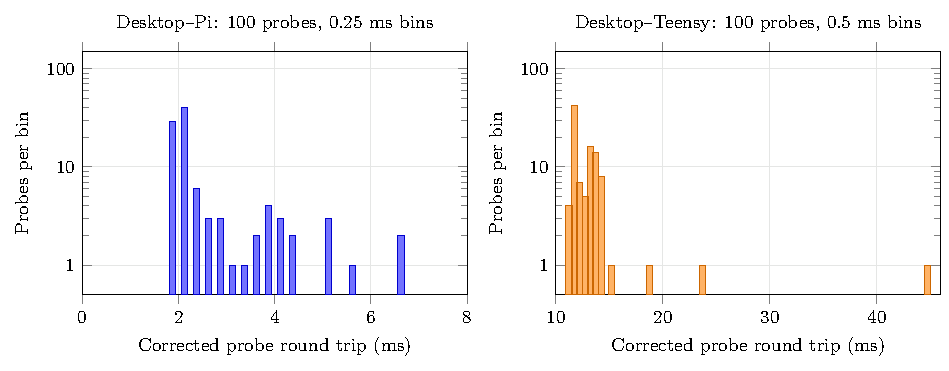
\includegraphics[width=.95\linewidth]{figures/desktop_clock/calibration_histograms.pdf}
\caption{Stale. Startup clock-calibration probes for the 50\,Hz reference run, September 27, 2026. Turnaround between the responder's receive and reply timestamps is subtracted from Desktop's send-to-receive interval. The panels have different horizontal scales and bin widths; logarithmic counts show all tails. These are observed probe round trips, not distributions of the unknown true clock offset.}
\label{fig:desktop-clock-probes}
\end{figure}

\subsubsection{From Aligned Timestamps to Control-Loop Latency}
For each acknowledged motor command, identify its originating sensor sample. Let $T_s$ denote Teensy's ADC-start time, $D_r$ Desktop's sensor-receipt time, $D_c$ Desktop's completed-target computation, and $T_r$ Teensy's complete motor-command receipt. Using one local clock-map estimate across this short cycle,
\begin{align}
 L_{T\to D}&=D_r-\widehat D(T_s), & C_D&=D_c-D_r,\\
 L_{D\to T}&=\widehat D(T_r)-D_c, & R&=T_r-T_s,\\
 S&=1000/f-R &&\text{(all durations in ms; $f$ in Hz).}
\end{align}
The offline code uses a common offset at the cycle midpoint, with a drift allowance across the cycle, so $L_{T\to D}+C_D+L_{D\to T}=R$ per matched row. Marginal medians or quartiles need not add. Forward latency starts at ADC acquisition, includes the three conversions (about 0.05\,ms), UART and network delivery; it is not wire-only transmission. Reverse latency ends when Teensy has received the complete target, before motor-output application. ACK return delivery to Desktop is excluded from $R$. Spare $S$ is the time remaining until the next sampling tick at target receipt, not CPU idle time; negative values are retained.

During offline analysis, pre/post GPIO-fit bounds are intersected at each cycle and combined with nearby Desktop--Pi network probes within a 2\,s window. The implementation includes the 100\,$\mu$s GPIO allowance, 50\,ppm GPIO-fit extrapolation allowance, a 2000\,ppm Desktop--Pi relative-rate guard, a 2\,$\mu$s network timestamp guard, and a small within-cycle drift/quantization allowance. Causality also requires both directional delays to be nonnegative. The interval midpoint gives the plotted estimate and its half-width gives conditional uncertainty. Offset errors shift the two directional estimates in opposite directions; a narrow latency histogram cannot rule out a fixed clock-offset bias. The raw Teensy round trip and spare are independent of that offset uncertainty.

\subsubsection{Message Sizes and Sampling-Rate Comparison}
\label{sec:message-sizes}
The 25, 50 and 100\,Hz recordings used the same message formats. Pi translates between ASCII records on the Teensy UART and binary packets on the Desktop LAN; a message therefore has a different size on each link. The three ADC values themselves occupy only 6 bytes as three unsigned 16-bit integers. The two signed motor targets occupy 4 bytes. Sequence identifiers, timestamps and diagnostic fields account for the rest.

\begin{table}[H]
\centering\small
\caption{Binary control messages, unchanged across the three sampling rates. The application frame is the complete UDP payload: a 24-byte protocol header plus the message body. UDP/IP and Ethernet/Wi-Fi framing are excluded.}
\label{tab:control-payloads}
\begin{tabular}{@{}llll@{}}
\toprule
Message and direction & Body (bytes) & Header + body (bytes) & Main contents \\
\midrule
SENSOR, Pi $\to$ Desktop & 58 & 82 & 3 ADCs, IDs, timestamps, drop count \\
COMMAND, Desktop $\to$ Pi & 12 & 36 & Source sample ID, left/right targets \\
STATUS, Pi $\to$ Desktop & 51 & 75 & State, acknowledged IDs, times, targets, counters \\
\bottomrule
\end{tabular}
\end{table}

The 24-byte header contains magic/version, message type, body length, session ID and sender sequence. At one SENSOR and one COMMAND per sample, their combined application traffic is 2.95, 5.90 and 11.80\,kB/s at 25, 50 and 100\,Hz, respectively (1\,kB = 1000 bytes). STATUS messages, clock probes, startup traffic and network framing add further traffic. These are nominal rate budgets; coalescing and stopping can reduce the actual command count. Pi forwards each ADC triplet together, not as three separate packets.

On UART, a sensor record is
\begin{verbatim}
S sequence start_us end_us ring_drops A B C\n
\end{verbatim}
and a motor record is \texttt{MOTORST left right\textbackslash n}. Here \texttt{\textbackslash n} denotes one LF byte; the field names are replaced by decimal values. Sizes include the command text, spaces, signs, all decimal digits and LF. They vary with sensor values, sequence number, timestamp magnitude and motor targets; the sampling rate does not directly set the byte count. Table~\ref{tab:uart-payloads} reconstructs their lengths from each run's complete UART audit log.

\begin{table}[H]
\centering\small
\caption{Unpadded UART records at 115200 baud, 8N1. Rate is in Hz; byte counts are median [minimum--maximum], including LF. Wire time is calculated for the median length, not measured end-to-end latency. Counts include all logged sensor records and dispatched motor commands, so they differ from matched timing-cycle counts.}
\label{tab:uart-payloads}
\begin{tabular}{@{}rrrrrrr@{}}
\toprule
Rate & Samples & Sensor bytes & Sensor wire (ms) & Commands & Motor bytes & Motor wire (ms) \\
\midrule
25 & 199 & 41 [39--43] & 3.56 & 198 & 17 [15--18] & 1.48 \\
50 & 399 & 40 [36--41] & 3.47 & 393 & 17 [15--18] & 1.48 \\
100 & 799 & 42 [40--43] & 3.65 & 770 & 17 [15--18] & 1.48 \\
\bottomrule
\end{tabular}

\end{table}

Each UART byte needs 10 serial bits (start, eight data, stop), giving 11,520 bytes/s per direction on this full-duplex link. The median sensor record therefore occupies about 3.5--3.6\,ms on the wire, compared with 1.48\,ms for the median 17-byte motor command. UART acknowledgements and clock traffic are additional. Serialization alone already contributes about 2\,ms more in the sensor direction. These wire times exclude ADC acquisition, software scheduling, buffering, parsing and LAN delivery, which are included in the observed control-loop intervals below.

\begin{table}[H]
\centering\small
\caption{Stale. Moving-run timing results from September 27 with the payloads above; the final row is the separate padded-command experiment. Directional columns and round trip are medians in ms; $u$ is the maximum per-cycle conditional one-way uncertainty in ms, rounded upward to 0.1\,ms. Cycles are complete matched observations, not all issued commands.}
\label{tab:desktop-clock-runs}
\begin{tabular}{@{}lrrrrrr@{}}
\toprule
Run & Active (s) & Cycles & $T\to D$ & $D\to T$ & Round trip & Max. $\pm u$ \\
\midrule
25 Hz & 7.9 & 198 & 5.4 & 2.7 & 8.2 & 2.4 \\
50 Hz & 8.0 & 392 & 5.2 & 2.7 & 8.1 & 2.6 \\
100 Hz & 8.0 & 770 & 5.6 & 2.6 & 8.3 & 2.4 \\
50 Hz, padded & 4.0 & 186 & 5.4 & 4.8 & 10.3 & 2.4 \\
\bottomrule
\end{tabular}

\end{table}

The original 25, 50 and 100\,Hz jobs all completed their requested 8\,s duration normally (the measured active interval excludes arming overhead). Sampling periods were exactly 40, 20 and 10\,ms in the recorded Teensy timestamps, with no missing sample slots. Median transport intervals remained similar across rates: 5.2--5.6\,ms from Teensy sampling to Desktop receipt, and 2.6--2.7\,ms from Desktop computation completion to Teensy target receipt. Desktop computation itself had medians 0.010, 0.013 and 0.013\,ms at 25, 50 and 100\,Hz. The median sample-to-target round trip was 8.1--8.3\,ms; changing the sample period did not scale this latency. Median spare time at target receipt was 31.8, 11.9 and 1.7\,ms, respectively. The robot started at different track positions, so these runs do not isolate sampling rate as the cause of small timing differences.

The GPIO-plus-network startup uncertainty grows to approximately $\pm2.3$--$\pm2.5$\,ms at the least-constrained cycles in these recordings because the probe distances and drift allowances differ. The startup $\pm1.4$\,ms figure must not be reused as a fixed uncertainty for every video frame. The later standalone wired Desktop--Pi calibration belongs to a different session and does not retroactively reduce these recordings' uncertainty.

\begin{figure}[H]
\centering
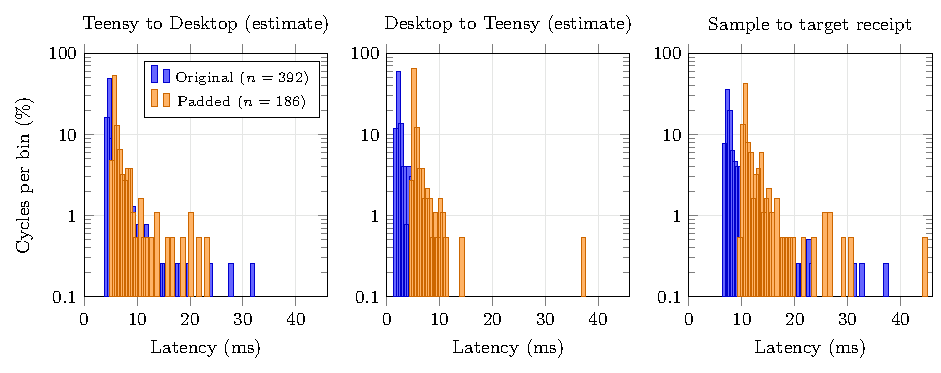
\includegraphics[width=\linewidth]{figures/desktop_clock/latency_histograms.pdf}
\caption{Stale. Control-loop latency at 50\,Hz, September 27, 2026, before and after padding the motor UART message. Histograms use common 0.5\,ms bins, normalized by each run's matched-cycle count, with logarithmic vertical scales and all outliers included. Adjacent colored bars represent the same bin. The first two panels depend on clock alignment; the third uses only Teensy's clock. The padded run stopped early and used a different track segment, so this is not a controlled steering-performance comparison.}
\label{fig:desktop-clock-latency}
\end{figure}

\subsubsection{Testing the Directional Asymmetry by Padding UART Commands}
At 115200 baud, 8N1, every byte takes $10/115200$\,s on the UART wire. In the original recordings, sensor records typically used 40--42 bytes, versus about 17 bytes for a motor command. The optional Pi switch \texttt{--match-motor-wire-size} prefixes a signed motor magnitude with zeros, preserving its value while matching the complete command's length, including LF, to its originating sensor record. Desktop UDP payloads, motor policy and firmware are unchanged; the switch defaults off.

The padded 50\,Hz run verified exact corresponding lengths and unchanged targets for all 186 dispatched commands; all 186 were acknowledged. The median predicted added serial time was 2.170\,ms. Relative to the earlier 50\,Hz reference, median round trip increased from 8.098 to 10.313\,ms, a 2.215\,ms increase. Pi-dispatch-to-Teensy-receipt timing, computed with the GPIO map and independent of Desktop offset, increased from 1.568 to 3.716\,ms. These changes closely support the UART serialization explanation. The remaining difference between directional estimates does not establish a network asymmetry within their uncertainty.

The padded job ended after 4.045\,s when the 100\,ms freshness safeguard expired. Pi acknowledged STOPALL and confirmed motor standby; Desktop's separate cleanup STOP was not acknowledged. Two pending targets were replaced at Pi and three issued commands were not accepted there. The exact network/host cause of the freshness gap was not identified, and no UART command or ACK loss was observed. The histogram includes the full captured active interval rather than presenting this as a completed 8\,s run.

\subsubsection{Software and Reproducing These Figures}
\begin{sloppypar}
The current measurement programs are C++17: \path{lineFollowerDistributed/clock_probe.cpp} on both machines and \path{gpio_clock.cpp} on the Pi, launched by \texttt{onDesktop/runClocksCalib}, which saves only the summary in Section~\ref{sec:clock-method}. \path{controller.cpp} and \path{operator.cpp} run the robot and do not collect this clock delay. Teensy uses the shared Arduino C++ firmware described above. These implementations use direct GPIO/UART/socket interfaces and avoid Python interpreter and garbage-collection work in the timing path. C++ does not eliminate OS scheduling or Wi-Fi delays. The four recordings and figures below are stale September 27 results; the current command does not write those archives.
\end{sloppypar}

Offline Python scripts from the earlier Desktop package join sample/command identities and timestamps: \path{prepare_stats_video.py}, \path{clock_alignment.py} and \path{integrated_clock_analysis.py}. The resulting per-cycle \path{timing_cycles.csv} contains the directional estimates, their bounds, compute time, round trip and spare. Those scripts render the September telemetry movies. The current recording is Appendix~\ref{app:telemetry-video}; its Swift renderer draws the banner and does not acquire control-loop timestamps.

The plotting script \path{docs/tools/plot_desktop_clock.py} uses Python's standard library to read the archived JSON, writes raw derived samples and histogram bins, and generates PGFPlots sources. Its default input is the sibling \path{2026_lineFollowerOperator/} directory; an alternate package root can be passed as an argument. Source paths and SHA-256 hashes are saved in \path{docs/figures/desktop_clock/sources.json}. The four input recordings under the operator's \path{out/} are:
\begin{itemize}
\item \path{integrated_25hz_20260927_205834};
\item \path{integrated_50hz_20260927_203812};
\item \path{integrated_100hz_20260927_205707};
\item \path{integrated_padded_50hz_20260927_212141}.
\end{itemize}
Reproduce the figures from the robot repository root:
\begin{verbatim}
python3 docs/tools/plot_desktop_clock.py
cd docs/figures/desktop_clock
pdflatex -halt-on-error calibration_histograms.tex
pdflatex -halt-on-error latency_histograms.tex
\end{verbatim}

\clearpage
\subsection{Standalone Desktop--Pi Clock-Offset Measurement}
\label{sec:standalone-desktop-pi}
The September 28 experiment isolates the Desktop--Pi part of the clock map. It compares a temporary wired Pi connection with the normal Pi Wi-Fi connection, without operating the motors or accessing Teensy. It measures clock offset and network round trip; it does not directly measure either one-way delay. All results in this subsection belong to this standalone session, not to the September 27 moving runs.

\subsubsection{Connections and Acquisition}
Figure~\ref{fig:desktop-pi-clock-network} shows the actual arrangement. Desktop remains wired to an ASUS LAN port, and an additional cable connects Pi to another ASUS LAN port. Pi Wi-Fi remains on AirBears 3. Desktop keeps its home-router Wi-Fi connection for Internet access. The Pi Ethernet address \texttt{10.0.0.24} was assigned by DHCP and may change; the existing Desktop \texttt{10.0.0.2} and Pi Wi-Fi \texttt{10.0.0.149} reservations remain in use. This is Ethernet through ASUS, not a direct Desktop--Pi cable.

\begin{figure}[H]
\centering
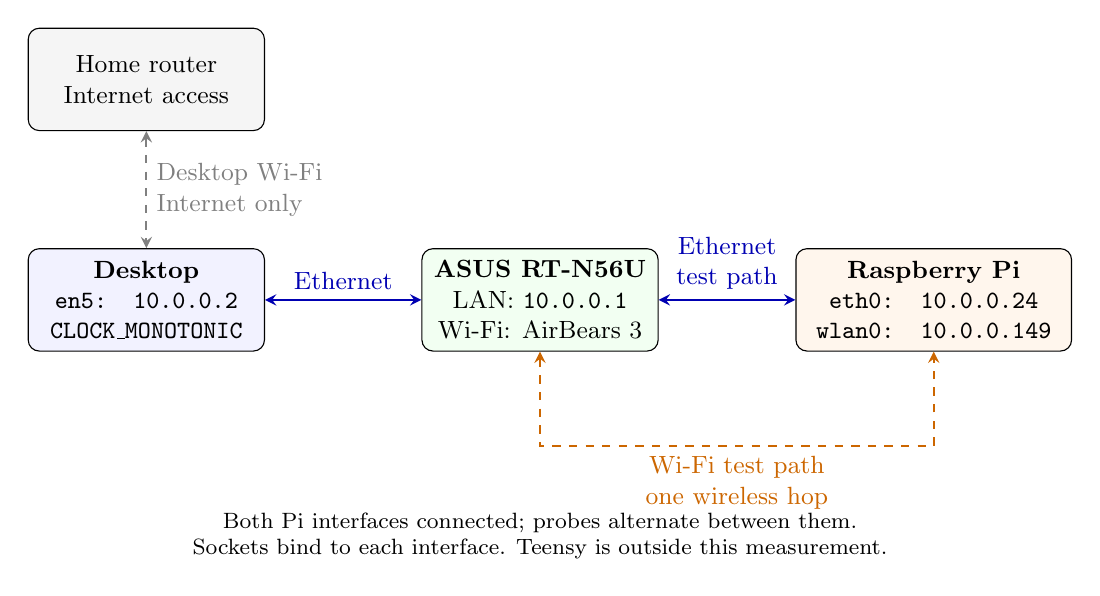
\begin{tikzpicture}[font=\small,box/.style={draw,rounded corners,align=center,minimum width=3cm,minimum height=1.3cm},link/.style={<->,thick,>=stealth}]
\node[box,fill=blue!5] (desktop) at (0,0) {\textbf{Desktop}\\\texttt{en5: 10.0.0.2}\\\texttt{CLOCK\_MONOTONIC}};
\node[box,fill=green!5] (asus) at (5,0) {\textbf{ASUS RT-N56U}\\LAN: \texttt{10.0.0.1}\\Wi-Fi: AirBears 3};
\node[box,fill=orange!7,minimum width=3.5cm] (pi) at (10,0) {\textbf{Raspberry Pi}\\\texttt{eth0: 10.0.0.24}\\\texttt{wlan0: 10.0.0.149}};
\node[box,fill=gray!8] (home) at (0,2.8) {Home router\\Internet access};
\draw[link,dashed,gray] (home) -- node[right,align=left] {Desktop Wi-Fi\\Internet only} (desktop);
\draw[link,blue!70!black] (desktop) -- node[above] {Ethernet} (asus);
\draw[link,blue!70!black] (asus.east) -- node[above,align=center] {Ethernet\\test path} (pi.west);
\draw[link,dashed,orange!80!black] (asus.south) -- ++(0,-1.2) -| node[pos=.25,below,align=center] {Wi-Fi test path\\one wireless hop} (pi.south);
\node[align=center,font=\footnotesize] at (5,-3.0) {Both Pi interfaces connected; probes alternate between them.\\Sockets bind to each interface. Teensy is outside this measurement.};
\end{tikzpicture}

\caption{Standalone clock-offset experiment. The wired and wireless Pi paths are measured separately while both remain connected. The Pi Ethernet link negotiated 100\,Mb/s full duplex. Desktop's home Wi-Fi carries Internet traffic, not the measurement probes.}
\label{fig:desktop-pi-clock-network}
\end{figure}

The standalone package is \path{2026_measure_pi_desktop_clock/} on Desktop, alongside the robot and operator packages. Its C++17 \texttt{clock\_probe} executable runs on both processors; Pi's copy is under \path{/home/pi/robot0/measure_pi_desktop_clock/}. Python launches the processes and analyzes saved data, outside the timestamp-critical path. C++ provides direct socket and timestamp-control access without an interpreter in the acquisition loop; it does not make either OS deterministic.

Two Pi UDP servers bind explicitly to \texttt{eth0} and \texttt{wlan0}, using ports 53120 and 53121. Desktop binds to \texttt{en5}. Incoming interface indices are checked, preventing a nominal Wi-Fi reply from silently taking Ethernet. Probes alternate between paths at approximately 20 probes/s/path, reversing pair order. Each request/reply application frame is 192 bytes, with session, probe and server-instance identifiers plus timestamps and diagnostics. This size differs from the robot's 82/36-byte SENSOR/COMMAND pair.

\subsubsection{Timestamp Method and Uncertainty}
For each exchange, $D_1$ is Desktop send time, $P_2$ Pi receive time, $P_3$ Pi reply time and $D_4$ Desktop receive time. Both receivers use kernel software receive timestamps. Desktop transmission is timestamped immediately before the application sends. Pi Ethernet uses a kernel software transmit timestamp matched by packet ID and returned in a follow-up datagram; $D_4$ still refers to the original reply. Pi's Wi-Fi driver does not advertise software transmit timestamping, so that path uses an application send timestamp. Thus the link comparison also includes different Pi transmit boundaries.

The Linux \href{https://docs.kernel.org/networking/timestamping.html}{socket timestamping interface} supplies receive/transmit metadata and packet IDs for matching transmit timestamps. Neither tested Pi interface exposes a hardware PTP clock; this experiment uses no NIC hardware timestamps. Kernel realtime timestamps are explicitly converted to each host's \texttt{CLOCK\_MONOTONIC} through nearby bracketed clock reads. Conversion and quantization allowances are retained in the uncertainty budget; clocks are never set or reset.

Here the displayed sign is $\psi=\text{Desktop}-\text{Pi}=-\phi$, giving positive values for this boot pair. Causality gives
\begin{equation}
 D_1-P_2\leq\psi\leq D_4-P_3,
 \qquad R_{DP}=(D_4-D_1)-(P_3-P_2).
\end{equation}
Pi turnaround is removed from the corrected round trip. The midpoint estimates offset; the half-width bounds the unknown directional asymmetry under the clock assumptions. The analysis expands each interval for timestamp mapping, quantization and an assumed 2000\,ppm rate guard across the probe. It does not divide latency equally between the two directions and call the result exact.

One-second window intersections additionally use a stated 50\,ppm rate allowance, with 2000\,ppm sensitivity results retained. A separate affine fit permits constant relative drift with at most 10\,$\mu$s model deviation over the run. These are conditional models, not verified oscillator specifications. A narrow histogram or a large sample count cannot remove an unknown fixed directional bias.

\subsubsection{Results and Interpretation}
The idle capture lasted 120\,s with 2400 probes per path; a second 60\,s capture used one busy C++ thread on Pi's single core and 1200 probes per path. All 7200 probes were valid, with no missing/rejected replies or Ethernet transmit-timestamp matching failures. Both runs used the same Pi boot ID. The load test represents CPU contention, not a full moving-robot workload.

\begin{table}[H]
\centering\small
\caption{Standalone Desktop--Pi results, September 28. All times are ms. The final column is the narrowest expanded individual-probe offset interval half-width, at that probe's instant; it is not a guaranteed uncertainty throughout a later job.}
\label{tab:standalone-desktop-pi}
\begin{tabular}{@{}llrrrr@{}}
\toprule
Condition & Pi link & Probes & RTT min. & RTT median & Best $\pm u$ \\
\midrule
Idle, 120 s & Ethernet & 2400 & 0.521 & 0.994 & 0.266 \\
Idle, 120 s & Wi-Fi & 2400 & 1.403 & 1.996 & 0.706 \\
CPU load, 60 s & Ethernet & 1200 & 0.504 & 0.971 & 0.257 \\
CPU load, 60 s & Wi-Fi & 1200 & 1.365 & 2.003 & 0.687 \\
\bottomrule
\end{tabular}

\end{table}

\begin{figure}[H]
\centering
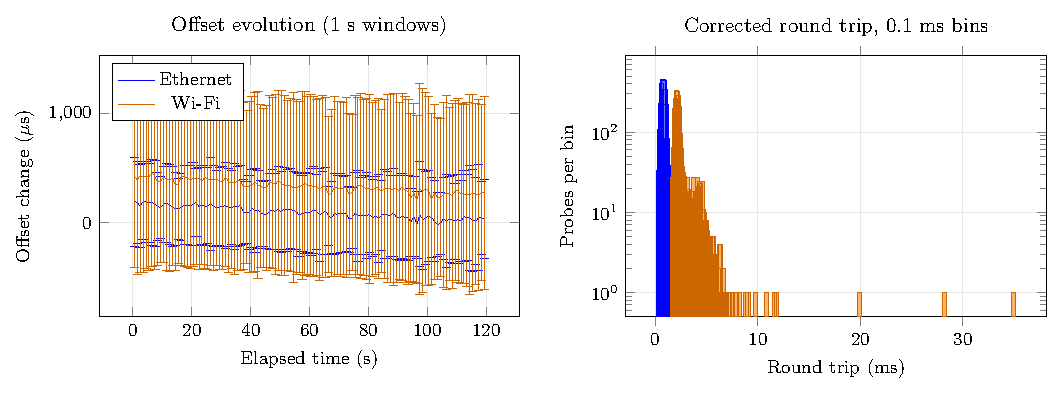
\includegraphics[width=\linewidth]{figures/pi_desktop_clock/20260928_073819_idle_plots.pdf}
\caption{Idle experiment: offset evolution and corrected round-trip distribution. The left panel subtracts one constant offset and plots one-second interval midpoints with conditional error bars using the 50\,ppm window assumption. The right panel includes all observed round trips in 0.1\,ms bins with logarithmic counts. Offset spread is not absolute accuracy.}
\label{fig:standalone-clock-results}
\end{figure}

Ethernet gave about $\pm0.26$--$\pm0.27$\,ms offset bounds, versus $\pm0.69$--$\pm0.71$\,ms over the Pi Wi-Fi path. The idle Ethernet affine estimate at elapsed 59.990\,s was Desktop minus Pi $=1118378.889885639$\,s $\pm0.270$\,ms under its model. The large positive value is the difference between clock origins, not a network delay. Sub-0.1\,ms absolute accuracy has not been demonstrated. The observed Ethernet median RTT was about 1\,ms, versus about 2\,ms on Wi-Fi; these are round trips of the standalone probes, not motor-control cycles.

Combining a fresh wired bound with the assumed 0.1\,ms GPIO allowance suggests a Desktop--Teensy uncertainty floor of roughly $\pm0.36$--$\pm0.37$\,ms before extrapolation, fitting and other mapping allowances. This is a prospective budget, not a measured integrated result. A cable removal does not itself reset the monotonic clocks, but subsequent drift needs a validated holdover model; 1\,ppm rate error alone accumulates 0.06\,ms per minute. No untethered holdover test was performed. A reboot invalidates the old calibration. These measurements cannot be retroactively applied to the earlier robot runs or interpreted as a reduction in their physical communication delay.

\begin{sloppypar}
Raw integer-nanosecond timestamps, reports and plots are in the standalone package's \path{out/20260928_073819_idle/} and \path{out/20260928_074049_cpu_load/}. The latest analyzed summary is \path{out/desktop_pi_clock.latest.json}. \texttt{run\_measurement.py} launches acquisition; \texttt{analyze.py} and \texttt{affine\_bounds.py} produce the intervals and plots. This report's copied figures, source hashes and derived tables are under \path{docs/figures/pi_desktop_clock/}; reproduce the tables with \path{docs/tools/report_pi_desktop_clock.py}.
\end{sloppypar}

\subsection{Available Cycle Time and Smaller-Message Options}
\label{sec:timing-budget}
\subsubsection{What ``Free'' Time Is Supported by the Measurements?}
For the existing robot, the defensible quantity is \emph{spare time at target receipt}: $S=1000/f-(T_r-T_s)$ in ms. Both timestamps are on Teensy, so Desktop clock-offset uncertainty does not enter this subtraction. Better alignment improves the separation into forward and reverse delay; it neither creates more spare time nor changes the already measured round trip. The measurements stop at complete target receipt, before motor-output application. They therefore do not establish CPU idle time or an exact interval from motor application to the next ADC tick. The spare-time numbers in this subsection are the stale September moving runs.

\begin{table}[H]
\centering\small
\caption{Stale. Observed spare time in the original unpadded moving runs. Quartiles are in ms. Late means the target arrived after the next nominal sample deadline; the denominator includes only complete matched cycles.}
\label{tab:spare-budget}
\begin{tabular}{@{}rrrrrr@{}}
\toprule
Rate (Hz) & Period (ms) & Spare Q1 & Spare median & Spare Q3 & Late / matched cycles \\
\midrule
25 & 40 & 30.9 & 31.8 & 32.0 & 0/198 (0.0\%) \\
50 & 20 & 10.4 & 11.9 & 12.3 & 10/392 (2.6\%) \\
100 & 10 & 0.5 & 1.7 & 2.1 & 156/770 (20.3\%) \\
\bottomrule
\end{tabular}

\end{table}

The most representative measured margins are therefore approximately \textbf{32\,ms at 25\,Hz, 12\,ms at 50\,Hz and 1.7\,ms at 100\,Hz}. The 100\,Hz run had 156/770 matched targets arrive late, about 20\%; a positive median is not a guaranteed computational budget. At 50\,Hz, 10/392 were late (2.6\%); none of the 198 matched 25\,Hz cycles were late. These short runs at different track positions do not prove long-term deadline reliability. Extra Desktop computation consumes approximately the same amount of spare time per cycle if other delays stay unchanged; it can also change queuing. New compute workloads must be checked against tails, not just these medians.

\subsubsection{ADC and Motor Resolution}
The current ADC already produces values in 0--1023, i.e. 10 useful bits per channel. Three losslessly packed channels need 30 bits, fitting in 4 bytes instead of the current six binary UDP bytes. Dropping three LSBs gives $q=a\mathbin{\gg}3$ in 0--127: seven bits/channel, or 21 bits in 3 bytes. Relative to lossless packing, this sacrifices precision to save only \emph{one additional byte per triplet}. Truncation reconstructed as $8q$ underestimates by 0--7 ADC counts; using the bin midpoint removes that systematic downward reconstruction choice but still leaves quantization error. The light thresholds and noise calibration must use consistent units. Recorded steering has not yet been replayed or driven with this quantization, so its effect near tape-detection thresholds is unverified.

Motor values are PWM targets, not measured speeds. The existing full range $-255$ to $+255$ needs nine bits per wheel, or 18 bits for both, packable into 3 bytes without loss. Six bits of \emph{magnitude} plus a direction bit gives 0--63 magnitudes in each direction, fitting each wheel in one byte. Mapping magnitude to the configured PWM maximum $M$ gives a step of about $M/63$: about 4 PWM counts at $M=255$, or 2 at $M=128$. Six bits total, including sign, would be coarser. It is plausible that six magnitude bits suffice for this toy controller, but these data do not establish the minimum usable resolution; low-speed starting and tight-turn behavior need checking. Again, reduced precision saves only one byte beyond losslessly packing both targets. Exact zero and the configured PWM limit must be preserved.

\subsubsection{Headers and Status}
The present LAN application header is \textbf{24 bytes (192 bits)}, not 24 or 26 bits. It contains 4-byte magic, 1-byte version, 1-byte type, 2-byte body length, 8-byte session and 8-byte sender sequence. There is no requirement for a 26-bit sensor header. A 24--26-bit total header cannot retain the existing independent session and sequence fields; reducing it that far changes the stale-command and reset-detection design. The serial ASCII records do not use this LAN header at all.

A possible LAN revision could use a 12-byte application header: version/type 1 byte, flags 1 byte, length 2 bytes, job token 4 bytes and sequence 4 bytes. The job token must be newly negotiated and bound to the active peer, with explicit rollover and old-session rejection rules; it is not authentication. A shorter session field has a higher collision risk than the current 64-bit field. UDP already provides datagram boundaries, but its \href{https://www.rfc-editor.org/rfc/rfc768}{own transport header} and the IP/link headers remain. Application compression cannot remove those headers, Wi-Fi contention or OS scheduling latency.

With that header and job-relative timestamps, a compact lossless SENSOR could occupy 23 bytes: header 12, sample-start time 4, ADC duration 2, packed ADCs 4 and diagnostic flags 1. Its header sequence identifies the sample. A COMMAND could occupy 19 bytes: header 12, source sample reference 4 and packed targets 3. Pi-side receipt timestamps and full counters would be kept in local logs for later joining. This illustrative 42-byte sensor/command pair replaces 118 bytes, saving 76 application bytes per cycle, or 1.90, 3.80 and 7.60\,kB/s at 25, 50 and 100\,Hz. These are design budgets, not implemented packets; clock-epoch, sequence and log-joining rules must change together.

STATUS can separate essential feedback from verbose diagnostics. Keep immediate stop/fault reporting and command receipt confirmation; send cumulative counters and repeated configuration at a lower rate, for example 5\,Hz. An illustrative 25-byte compact UDP status is a 12-byte header plus acknowledged sample/command reference (4), Teensy receipt time relative to the job (4), applied target pair (3), and state/flags (2). It retains the receipt timestamp needed for timing. Pi-local dispatch times and other diagnostics can remain in the Pi log and be joined offline by ID. A normal receipt report may be piggybacked on subsequent sensor traffic only if its added delay is acceptable; waiting for the next sample can delay that report by up to 10, 20 or 40\,ms. Critical stop/fault feedback should not wait. These changes reduce telemetry traffic but must not erase command-loss accounting or make feedback appear instantaneous.

Reducing each per-command STATUS from 75 to 25 bytes saves another 1.25, 2.50 and 5.00\,kB/s at those three nominal rates, before adding the slower diagnostic stream. This is a bandwidth saving; the ACK/status return path is outside the sample-to-target-receipt definition of round trip, so it cannot simply be subtracted from that measured latency.

\subsubsection{Estimated Communication Savings: Binary UART First}
The clearest near-term saving is a binary UART protocol, because every removed byte saves $10/115200$\,s $=0.0868$\,ms of serialization. The padded-message experiment already supports this mechanism. As a concrete \emph{unimplemented} size budget, consider a fixed-length serial frame with 2-byte sync marker, 1-byte type/version, 4-byte job token, 2-byte sample sequence and 2-byte CRC: 11 bytes of common framing/check fields. A single command per source sample uses that sample sequence as its reference.

\begin{table}[H]
\centering\small
\caption{Illustrative binary UART sizes, including framing and CRC. These proposed formats have not been installed or measured.}
\begin{tabular}{@{}lrrl@{}}
\toprule
Record & Full precision & Reduced precision & Fields beyond the 11-byte common part \\
\midrule
Sensor & 22 bytes & 21 bytes & Start time (4), ADC duration (2), ADCs (4 or 3), flags (1) \\
Motor target & 14 bytes & 13 bytes & Two packed targets (3 or 2) \\
\bottomrule
\end{tabular}
\end{table}

The four-byte microsecond time is relative to an agreed job epoch and wraps after 71.6\,min; sequence wraps after 655.36\,s at 100\,Hz. Unwrapping, reset detection, session changes and maximum accepted age must be specified explicitly. ADC duration preserves the acquisition-end timestamp; sequence gaps and flags can report sample loss, with full counters in diagnostics. CRC validation, resynchronization and bounded parsing are required for a serial byte stream. A CRC detects corruption; it does not authenticate commands. If multiple commands per sample or more diagnostics are needed, allocate additional fields rather than silently overloading IDs.

Relative to the recorded median sensor lengths of 41, 40 and 42 bytes and the 17-byte motor command, the lossless 22/14-byte proposal saves 22--23 bytes at 25/100\,Hz and 21 bytes at 50\,Hz. Table~\ref{tab:compact-projection} subtracts only that calculated serial time from the observed median round trip. It assumes all other delays remain unchanged, with no additional buffering or framing overhead; changes in CRC/parsing work, queues and ACK scheduling could alter the result.

\begin{table}[H]
\centering\small
\caption{Speculative binary-UART projection, not new measurements. Rate is Hz; times are ms. Bytes saved are per sensor-plus-command pair. The last column additionally drops three ADC LSBs and uses six-bit motor magnitudes, saving two further bytes (0.174\,ms per cycle).}
\label{tab:compact-projection}
\begin{tabular}{@{}rrrrrr@{}}
\toprule
Rate & Bytes saved & Wire saving & Projected round trip & Projected spare & Spare, reduced precision \\
\midrule
25 & 22 & 1.91 & 6.3 & 33.7 & 33.9 \\
50 & 21 & 1.82 & 6.3 & 13.7 & 13.9 \\
100 & 23 & 2.00 & 6.3 & 3.7 & 3.9 \\
\bottomrule
\end{tabular}

\end{table}

Thus lossless binary UART could plausibly shorten the typical cycle by about \textbf{1.8--2.0\,ms}, leaving roughly 33.7, 13.7 and 3.7\,ms spare at 25, 50 and 100\,Hz. The proposed quantization adds only about 0.17\,ms to that saving; retaining sensor and motor precision initially is therefore attractive. Neither projection eliminates Wi-Fi/OS tails or demonstrates that 100\,Hz will always meet its deadline.

Shrinking only the UDP packets leaves the UART bottleneck unchanged. Even saving 100 network bytes is just 8\,$\mu$s of raw serialization on a 100\,Mb/s link, or 0.133\,ms at an illustrative 6\,Mb/s radio data rate, before link overhead. The actual Wi-Fi data rate and contention vary, so these are arithmetic examples, not measured savings. Smaller or less frequent STATUS packets may reduce queue pressure, but that gain is unmeasured. The measurements support prioritizing lossless UART packing, then compact headers/status, and only then evaluating whether reduced numerical precision is worthwhile.

